\documentclass[10pt]{../usamts}

\realname{Juni Kim}
\username{junikimm}
\usamtsid{38002}
\usamtsyear{35}
\usamtsround{1}

\begin{document}

\begin{solution}{1}
\begin{figure}[htbp]
    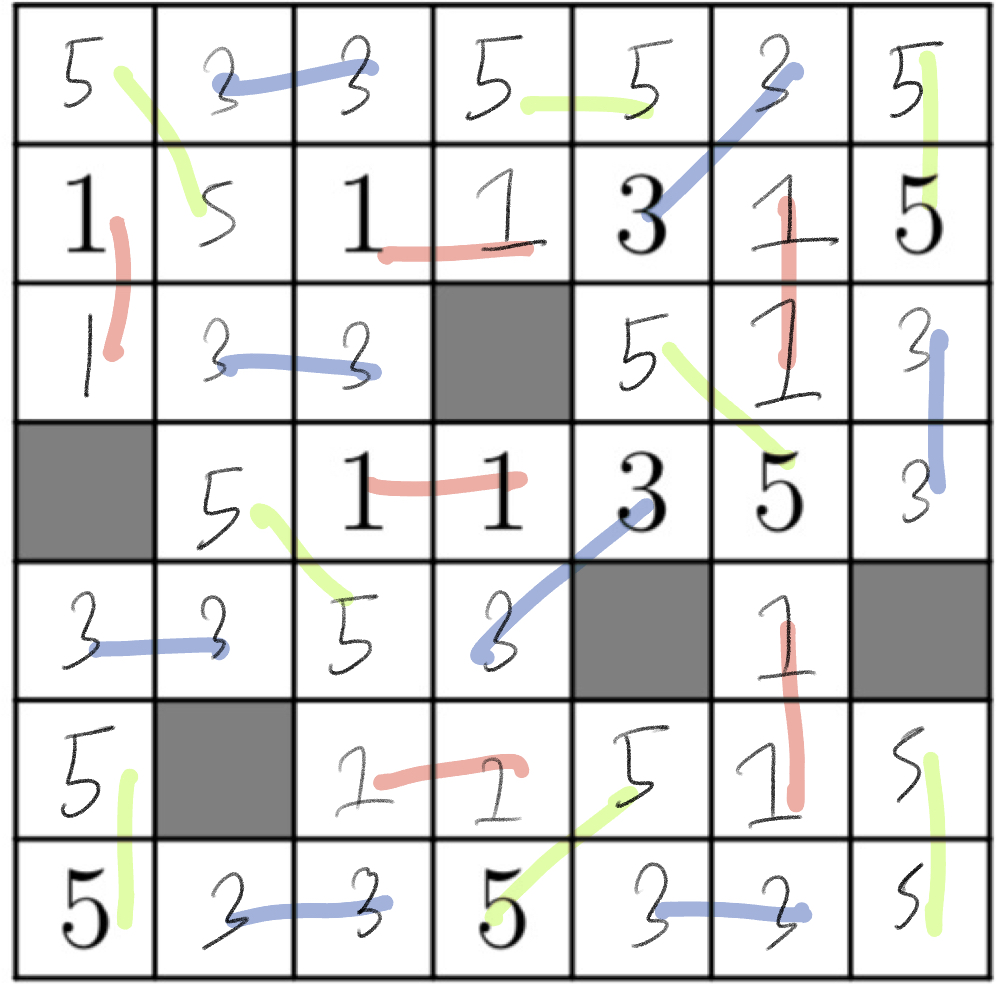
\includegraphics[width=4in]{p1.jpeg}
    \caption{We claim that this is a valid solution to the puzzle. The red highlights are pairs of touching ones, the blue highlights are pairs of touching threes, and the green highlights are pairs of touching fives.}
\end{figure}
\end{solution}

\begin{solution}{2}

Consider any permutation of the 101 numbers from 2024 to 2124 inclusive, arranged in the sequence $a_0, a_1 \dots a_{100}$. The concatenation of these 101 numbers can be represented as $\overline{a_{100} a_{99} \dots a_{1} a_{0}}$.

\begin{claim}
    $101\,|\,\overline{a_{100} a_{99} \dots a_{1} a_{0}}$
\end{claim}
\begin{proof}
    
    \begin{align*}
    \overline{a_{100} a_{99} \dots a_{1} a_{0}}
        &= \sum_{i=0}^{100} a_i \paren{10}^{4i} \\
        &\equiv \sum_{i=0}^{100} a_i (1)^i \mod 101 \because 10^4 \equiv 1 \mod 101\\
        &\equiv \sum_{i=0}^{100} a_i \mod 101 \\
        &\equiv (2124 - 2024 + 1) \cdot \frac{2024 + 2124}{2} \equiv 0 \mod 101 \\
        &\equiv 101 \cdot 2074 \mod 101 \\
        &\equiv 0 \mod 101
    \end{align*}
\end{proof}
\begin{claim}
    $\overline{a_{100} a_{99} \dots a_{1} a_{0}}$ is not prime.
\end{claim}
\begin{proof}
    Because
    $\overline{a_{100} a_{99} \dots a_{1} a_{0}}$ has 404 digits (with the first digit being nonzero), it is strictly greater than $10^{200}$, which itself is greater than 101. So, $\overline{a_{100} a_{99} \dots a_{1} a_{0}}$ has a divisor that is neither itself nor 1.
\end{proof}

\end{solution}

\begin{solution}{3}

\begin{definition}
    Let $h_i$ denote the height of the $i$th building from the right.
\end{definition}

\begin{definition}
    Consider a pair of two distinct buildings to be \textit{$k$-min roof-friendly} if and only if the pair is roof-friendly and the building with the shorter height is the $k$th building. 
\end{definition}
\begin{definition}
A \textit{right k-min roof-friendly pair} is a \textit{k-min roof-friendly pair} where the shorter building is to the right of the taller building in the pair.
\end{definition}

\begin{definition}
A \textit{left k-min roof-friendly pair} is a \textit{k-min roof-friendly pair} where the shorter building is to the left of the taller building in the pair.
\end{definition}

\begin{claim}
    The minimum possible number of \textit{roof-friendly} pairs is $\boxed{n-1}$.
\end{claim}

\begin{proof}
    Every adjacent pair of buildings has to be \textit{roof-friendly} because there are no buildings between them. Thus, the lower bound is the number of adjacent pairs of buildings, which is just $n-1$.
    
    This is easily achievable by letting $h_i = i$. Then, any two non-adjacent buildings cannot be roof-friendly. Between the $i$th and $j$th buildings where $i < i+1 < j$, the $i+1$th building exists. However, $h_{i+1} = i+1 > h_i = i$, so the $i$th and $j$th building are not roof-friendly.
\end{proof}

\begin{claim}
    A \textit{left k-min roof-friendly pair} exists if and only if there exists a building to the right of the $k$th building that is taller than it. Furthermore, there can only exist at most one such pair.
    \label{claim:kminleft}
\end{claim}

\begin{proof}
    Consider the $k$th building. Let there exist a building to its right that is taller than it. Then, we define the $l$th building as the leftmost building to the right of the $k$th building such that $h_l > h_k$. Then, the $k$th building and the $l$th building form a \textit{left k-min roof-friendly} pair because every building in-between is shorter than the $k$th building, which itself is shorter than the $l$th building. However, the $k$th building and the $\paren{l+x}$th building where $x > 0$ cannot form a roof-friendly pair because $h_l > h_k$ and $k < l < l+x$.
    
    If there are no buildings to the right of the $k$th building that are taller than it, then a \textit{left k-min roof-friendly pair} cannot be constructed by definition.
\end{proof}

\begin{claim}
    A \textit{right k-min roof-friendly pair} exists if and only if there exists a building to the left of the $k$th building that is taller than it. Furthermore, there can only exist at most one such pair.
    \label{claim:kminright}
\end{claim}

\begin{proof}
    This follows analogously by symmetry from Claim \ref{claim:kminleft}
\end{proof}

\begin{claim}
    The maximum possible number of \textit{roof-friendly pairs} is $\boxed{2n-3}$.
\end{claim}

\begin{proof}
     From claims \ref{claim:kminleft} and \ref{claim:kminright}, we conclude that the number of \textit{k-min roof-friendly pairs} is upper bounded by both the number 2 and the number of buildings that are taller than the $k$th building. So, the building with height $n$ cannot have any corresponding min roof-friendly pairs, and the building with height $n-1$ can have at most 1 corresponding \textit{min roof-friendly pair}.
    
    The number of roof-friendly pairs can be calculated by summing up all of the $i$-min roof-friendly pairs for $i$ between 1 and n. Thus, our upper bound is $2(n-2) + 1 = 2n-3$.
    
    We now show a construction exists. Let $h_1 = n$ and $h_i = i-1$ for all $i \ge 2$. The number of roof-friendly pairs between the 2nd and $n$th buildings, because they are ordered in ascending order, must be $n-2$. Now, we consider that the $1$st building (the tallest building) and the $i$th building are always a roof-friendly pair because the $2$nd, \dots $i-1$th buildings are all shorter than the $i$th building. So, this adds $n-1$ more roof-friendly pairs, leaving us with our final total of $2n-3$.
\end{proof}

\end{solution}

\begin{solution}{4}
WLOG, let $x \le y \le x^2$. Because $\sqrt{x} \le x^2$, we know that $x \ge 1$ and also $y \ge 1$. By Vieta's formulas, the roots of the following cubic polynomial must form a solution to the system of equations given in the problem:
\[
P(z) = z^3 - \frac{x + x^2 + x^4 + y + y^2 + y^4}{2}z^2 + \frac{x^3 + x^5 + x^6 + y^3 + y^4 + y^6}{2}z - \frac{x^7 + y^7}{2}
\]

It thus suffices to show that, given $1 \le x \le y \le x^2$, $P(z)$ must have three real roots with multiplicity. We first eliminate all the equality cases:

\begin{enumerate}
\item If $y=x$, we get the roots $(x, x^2, x^4)$.
    Verify this with the following WolframAlpha Query:
\begin{verbatim}
solve for z, z^3 - z^2 * (x + x^2 + x^4 + x + x^2 + x^4)/2
+ z*(x^3 + x^5 + x^6 + x^3 + x^5 + x^6)/2 - (x^7 + x^7)/2
\end{verbatim}
    
\item If $y=x^2$, we get the roots $(x^2, x^4, \frac{x^8 + x}{2})$.
    Verify this with the following WolframAlpha Query:
\begin{verbatim}
solve for z, z^3 - z^2 * (x + x^2 + x^4 + x^2 + x^4 + x^8)/2
+ z*(x^3 + x^5 + x^6 + x^6 + x^10 + x^12)/2 - (x^7 + x^14)/2
\end{verbatim}

\item If $x=1$, then $y=1$, and so $P(z) = z^3 - 3z^2 + 3z - 1 = (x-1)^3$, which has 1 as a triple root.
\end{enumerate}

From this point, let $1 < x < y < x^2$ because we covered every single case where this is not true. We now make the following claims:

%%%%%%%%%% CASE 1 %%%%%%%%%%
\begin{claim}
    $P(x) < 0$
    \label{claim:px}
\end{claim}
\begin{proof}
    $$P(x) = \frac{1}{2}\paren{x-y}\paren{x-y^2}\paren{x-y^4}$$
    Verify this equivalence with the following WolframAlpha Query (should return 0): 
    \begin{verbatim}
( (x^1)^3 - (x^1)^2 * (x+x^2+x^4 + y + y^2 + y^4)/2 
+ (x^1)^1 * (x^3 + x^5 + x^6 + y^3 + y^5 + y^6)/2 - (x^7 + y^7)/2 )
- 1/2 * (x-y)(x-y^2)(x-y^4)
    \end{verbatim}
    Now, we perform sign analysis:
    \begin{itemize}
        \item $x - y < 0 \impliedby y > x > 1$
        \item $x - y^2 < 0 \impliedby y > x > 1$
        \item $x - y^4 < 0 \impliedby y > x > 1$
    \end{itemize}
    This proves that $P(x)$ must be negative.
\end{proof}

%%%%%%%%%% CASE 2 %%%%%%%%%%
\begin{claim}
    $P(x^2) > 0$
    \label{claim:px2}
\end{claim}
\begin{proof}
    $$P(x^2) = \frac{1}{2} \paren{x^2-y}\paren{y^2 - x^2}\paren{y^4 - x^2}$$
    Verify this equivalence with the following WolframAlpha Query (should return 0): 
    \begin{verbatim}
( (x^2)^3 - (x^2)^2 * (x+x^2+x^4 + y + y^2 + y^4)/2 
+ (x^2)^1 * (x^3 + x^5 + x^6 + y^3 + y^5 + y^6)/2 - (x^7 + y^7)/2 )
- 1/2 * (x^2 - y)(y^2-x^2)(y^4-x^2)
    \end{verbatim}
    Now, we perform sign analysis:
    \begin{itemize}
        \item $x^2 - y > 0 \impliedby y < x^2$
        \item $y^2 - x^2 > 0 \impliedby y > x > 1$
        \item $y^4 - x^2 > 0 \impliedby y > x > 1$
    \end{itemize}
    This proves that $P(x^2)$ must be positive.
\end{proof}

%%%%%%%%%% CASE 3 %%%%%%%%%%
\begin{claim}
    $P(x^4) < 0$
    \label{claim:px4}
\end{claim}
\begin{proof}
    $$P(x^4) = \frac{1}{2} \paren{x^4-y} \paren{y^4 - x^4}\paren{y^2 - x^4}$$ 
    Verify this equivalence with the following WolframAlpha Query (should return 0): 
    \begin{verbatim}
( (x^4)^3 - (x^4)^2 * (x+x^2+x^4 + y + y^2 + y^4)/2 
+ (x^4)^1 * (x^3 + x^5 + x^6 + y^3 + y^5 + y^6)/2 - (x^7 + y^7)/2 )
- 1/2 * (x^4 - y)(y^4 - x^4)(y^2 - x^4)
    \end{verbatim}
    Now, we perform sign analysis:
    \begin{itemize}
        \item $x^4 - y > 0 \impliedby x^2 > y > 1$
        \item $y^4 - x^4 > 0 \impliedby x > y > 1$
        \item $y^2 - x^4 < 0 \impliedby 1 < y < x^2$
    \end{itemize}
    This proves that $P(x^3)$ must be negative.
\end{proof}

%%%%%%%%%% CASE 4 %%%%%%%%%%
\begin{claim}
    $P(x^2 + x^4 + x^8 + x^{14}) > 0$.
    \label{claim:pinfty}
\end{claim}
\begin{proof}
    Let $z = x^2 + x^4 + x^8 + x^{14}$. $x > 1$ implies $z > 1$.
    \begin{align*}
    P(z) &> P(z)/z^2 \\
         &> z - \frac{x+x^2+x^4+y+y^2+y^4}{2} - \frac{x^7+y^7}{2z^2} \\
         &> z - \frac{x+x^2+x^4+y+y^2+y^4}{2} - \frac{x^7+y^7}{2} \\
         &> z - (y + y^2 + y^4 + y^7) \\
         &> z - (x^2 + x^4 + x^8 + x^{14})
    \end{align*}
    Thus,  $P(x^2 + x^4 + x^8 + x^{14})$ is positive.
\end{proof}

\begin{claim}
    $P(z)$ has three real roots.
\end{claim}

\begin{proof}
    We use claims \ref{claim:px}, \ref{claim:px2}, \ref{claim:px4}, and \ref{claim:pinfty}.
    Because $P(z)$ is continuous everywhere in $\RR$, we can apply the intermediate value theorem.
    From this, we know that $P(z)$ has at least one root in each of the disjoint intervals $(x, x^2)$, $(x^2, x^4)$, and $(x^4, x^2 + x^4 + x^8 + x^{14})$; this implies that there are at least three distinct real roots. Since $P(z)$ is cubic and can have at most three roots, this implies that all of its roots are real.
\end{proof}

\end{solution}


%%%%%%%%%%%%%%%%%%%%%%%%%%
%%%%%%%%%%%%%%%%%%%%%%%%%%
%%%%%%%%%%%%%%%%%%%%%%%%%%
%%%%%%%%%%%%%%%%%%%%%%%%%%
%% THE GLORIOUS P5 BASH %%
%%%%%%%%%%%%%%%%%%%%%%%%%%
%%%%%%%%%%%%%%%%%%%%%%%%%%
%%%%%%%%%%%%%%%%%%%%%%%%%%
\begin{solution}{5}
First, we find the following areas for the white regions:

\newcommand{\showareacalc}[2]{
    &= \frac{h}{2}(b_1 + b_2) \\
    &= \paren{\cos{#1} - \cos{#2}}\paren{\sin{#1} + \sin{#2}} \\
    &= \cos{#1}\sin{#1} - \cos{#2} \sin{#2} + \sin{#2 - #1} \\
    &= \frac{1}{2}\paren{\sin{2 \cdot #1} - \sin{2 \cdot #2}} + \sin{\frac{2\pi}{13}}
}
\newcommand{\showtrianglebarea}{
    \frac{1}{2} \tan{\frac{2\pi}{13}} - \frac{1}{2} \sin{\frac{2\pi}{13}}
}

\newcommand{\sinthirteen}[1]{
    \sin{{\frac{#1\pi}{13}}}
}
\newcommand{\costhirteen}[1]{
    \cos{{\frac{#1\pi}{13}}}
}
\newcommand{\tanthirteen}[1]{
    \tan{{\frac{#1\pi}{13}}}
}

\newcommand{\expthirteen}[1]{
    e^{\frac{#1\pi}{13}}
}

\begin{align*} 
[A_1A_2A_3] \showareacalc{0}{\frac{2\pi}{13}} \\
[A_3A_4A_{11}A_{12}] \showareacalc{\frac{4\pi}{13}}{\frac{6\pi}{13}} \\
[A_5A_6A_{8}A_{10}] \showareacalc{\frac{8\pi}{13}}{\frac{10\pi}{13}} \\
    [A_7A_8B] &= \cos^2{\frac{\pi}{13}} \cdot \tan{\frac{2\pi}{13}} \\
              &= \frac{1 - \cos{\frac{2\pi}{13}}}{2} \cdot \frac{\sin{\frac{2\pi}{13}}}{\cos{\frac{2\pi}{13}}}\\
              &= \showtrianglebarea
\end{align*}

We now find the following areas for the gray regions:
\begin{align*}
[A_2A_3A_{12}A_{13}] \showareacalc{\frac{2\pi}{13}}{\frac{4\pi}{13}} \\
[A_4A_5A_{10}A_{11}] \showareacalc{\frac{6\pi}{13}}{\frac{8\pi}{13}} \\
[A_6A_7A_{8}A_{9}] \showareacalc{\frac{10\pi}{13}}{\frac{12\pi}{13}} \\
\end{align*}

The problem asks us to prove that
\begin{equation}
[A_1A_2A_3] + [A_3A_4A_{11}A_{12}] + [A_5A_6A_{8}A_{10}] + [A_7A_8B] = [A_2A_3A_{12}A_{13}] + [A_4A_5A_{10}A_{11}]+ [A_6A_7A_{8}A_{9}]
\end{equation}

First, we can cancel the three $\sin\frac{2\pi}{13}$ terms on each side:

\newcommand{\showsinsubtraction}[2] {
    \frac{1}{2}\paren{\sinthirteen{#1} - \sinthirteen{#2}}
}

\begin{align*}
    &\showsinsubtraction{0}{4} +
    \showsinsubtraction{8}{12} +
    \showsinsubtraction{16}{20} +
    \showtrianglebarea \\
    &=
    \showsinsubtraction{4}{8} +
    \showsinsubtraction{12}{16} +
    \showsinsubtraction{20}{24}
\end{align*}

Rearranging a lot of terms and using some identities, we get

\begin{align*}
    &\showtrianglebarea \\
    &= \sinthirteen{4} - \sinthirteen{8} + \sinthirteen{12} - \sinthirteen{16}
    + \sinthirteen{20} + \frac{-\sin0 - \sinthirteen{24}}{2} \\
    &= \sinthirteen{4} - \sinthirteen{5} + \sinthirteen{} + \sinthirteen{3}
    - \sinthirteen{6} + \frac{\sin0 + \sinthirteen{2}}{2}
\end{align*}

So, we need to prove that

\begin{equation}
    \frac{1}{2} \tanthirteen{2}
    = \sinthirteen{} + \sinthirteen{2} + \sinthirteen{3} + \sinthirteen{4} - \sinthirteen{5} - \sinthirteen{6}
\end{equation}

We compute $\sinthirteen{} + \sinthirteen{2} + \sinthirteen{3} + \sinthirteen{4}$.

\begin{align*}
    \sinthirteen{} + \sinthirteen{2} + \sinthirteen{3} + \sinthirteen{4}
    &=\Im\paren{\expthirteen{} + \expthirteen{2} + \expthirteen{3} + \expthirteen{4}} \\
    &= \Im\paren{1 + \expthirteen{} + \expthirteen{2} + \expthirteen{3} + \expthirteen{4}}\\
    &= \Im\paren{\frac{\expthirteen{5} - 1}{\expthirteen{} - 1}} \\
    &= \Im\paren{\frac{\paren{\costhirteen{5}-1} + i\sinthirteen{5}}{\paren{\costhirteen{}-1} + i\sinthirteen{}}} \\
    &= \Im\paren{\frac{\paren{\costhirteen{5}-1} + i\sinthirteen{5}}{\paren{\costhirteen{}-1} + i\sinthirteen{}}
    \cdot \frac{\paren{\costhirteen{}-1} - i\sinthirteen{}}{\paren{\costhirteen{}-1} - i\sinthirteen{}}}\\
    &= \frac{\sinthirteen{5}\costhirteen{}  - \sinthirteen{}\costhirteen{5} - \sinthirteen{5} + \sinthirteen{}}
    {2 - 2\costhirteen{}} \\
    &= \frac{\sinthirteen{} + \sinthirteen{4} - \sinthirteen{5}} {2 - 2\costhirteen{}}
\end{align*}

We now also compute $-\paren{\sinthirteen{5} + \sinthirteen{6}}\paren{2 - 2\costhirteen{}}$ using product to sum.

\begin{align*}
    \sinthirteen{5}\paren{-2 + 2\costhirteen{}} &= -2\sinthirteen{5} + \sinthirteen{4} + \sinthirteen{6} \\
    \sinthirteen{6}\paren{-2 + 2\costhirteen{}} &= -2\sinthirteen{6} + \sinthirteen{5} + \sinthirteen{7}
\end{align*}
\begin{align*}
    -\paren{\sinthirteen{5} + \sinthirteen{6}}\paren{2 - 2\costhirteen{}}
    &= -2\sinthirteen{6} + \sinthirteen{5} + \sinthirteen{7} -2\sinthirteen{5} + \sinthirteen{4} + \sinthirteen{6} \\
    &= \sinthirteen{4} - \sinthirteen{5} -\sinthirteen{6} + \sinthirteen{7}
\end{align*}

Therefore,
\[
-\sinthirteen{5} -\sinthirteen{6} = \frac{\sinthirteen{4} - \sinthirteen{5} -\sinthirteen{6} + \sinthirteen{7}}{2 - 2 \costhirteen{}}
\]

We now derive Equation \ref{eq:p5final}, which is logically equivalent to the problem statement.

\begin{equation*}
    \frac{1}{2} \tanthirteen{2} = \paren{\sinthirteen{} + \sinthirteen{2} + \sinthirteen{3} + \sinthirteen{4}} - \paren{\sinthirteen{5} + \sinthirteen{6}} \\
\end{equation*}

\begin{align*}
    \frac{\sinthirteen{} + \sinthirteen{4} - \sinthirteen{5}} {2 - 2\costhirteen{}}
    -\paren{\sinthirteen{5} + \sinthirteen{6}}
    &= \frac{\sinthirteen{} + \sinthirteen{4} - \sinthirteen{5}} {2 - 2\costhirteen{}} +\\
    & \frac{\sinthirteen{4} - \sinthirteen{5} -\sinthirteen{6} + \sinthirteen{7}} {2 - 2\costhirteen{}} \\
    &= \frac{\sinthirteen{} + 2\sinthirteen{4} - 2\sinthirteen{5} - \sinthirteen{6} + \sinthirteen{7}} {2 - 2\costhirteen{}} \\
\end{align*}

\begin{equation*}
    2 \times \frac{\sinthirteen{} + 2\sinthirteen{4} - 2\sinthirteen{5} - \sinthirteen{6} + \sinthirteen{7}} {2 - 2\costhirteen{}}
    = 2 \times \frac{1}{2} \frac{\sinthirteen{2}}{\costhirteen{2}} \\
\end{equation*}

\begin{equation}
    \costhirteen{2}\paren{\sinthirteen{} + 2\sinthirteen{4} - 2\sinthirteen{5} - \sinthirteen{6} + \sinthirteen{7}}
    = \sinthirteen{2}\paren{1 - \costhirteen{}}
    \label{eq:p5final}
\end{equation}

We now simplify the LHS. This is possible by using the fact that $\cos(a)\sin(b) = \frac{1}{2}\paren{\sin(b-a) + \sin(b+a)}$:

\begin{align*}
    \costhirteen{2}\paren{\sinthirteen{} + 2\sinthirteen{4} - 2\sinthirteen{5} - \sinthirteen{6} + \sinthirteen{7}}
    &= \frac{-\sinthirteen{} + \sinthirteen{3}}{2} + \\
    &\sinthirteen{2} + \cancel{\sinthirteen{6}} + \\
    &- \sinthirteen{3} -\cancel{\sinthirteen{7}} + \\
    &-\cancel{\frac{\sinthirteen{4}}{2}} + -\cancel{\frac{\sinthirteen{8}}{2}} +\\
    &+ \cancel{\frac{\sinthirteen{5}}{2}} + \cancel{\frac{\sinthirteen{9}}{2}} \\
    &= \boxed{-\frac{\sinthirteen{}}{2} - \frac{\sinthirteen{3}}{2} + \sinthirteen{2}}
\end{align*}

We now simplify the RHS with the product-to-sum formula.
\begin{align*}
    \sinthirteen{2}\paren{1 - \costhirteen{}}
    &= \boxed{\sinthirteen{2} - \frac{\sinthirteen{} + \sinthirteen{3}}{2}}
\end{align*}

Thus, the LHS equals the RHS, and Equation \ref{eq:p5final} is definitively true.
$\blacksquare$
\end{solution}

\end{document}
